We prove lower bounds to show that coming up with good streaming algorithms for approximate convex hulls is difficult.

\section{Streaming Model}

Given a stream/sequence of points $P$. A streaming algorithm $A$ is given $\epsilon$ in advance but is not given the size of the point stream $P$. As $A$ processes $P$ it maintains a subset $S$ of the points it has seen so far.
\\

The streaming algorithm $A$ is given the points in $P$ sequentially. Each time $A$ is given a point $p \in P$, $A$ can choose to add $p$ to $S$ (remembering $p$) or ignore $p$ (and permanently forget $p$). $A$ can also choose to delete points in $S$, in which case these points are permanently lost. The important part is that $A$ cannot go back in time and access points it did not keep.
\\

Typically we want $S$ to be an $\epsilon$-approximate convex hull of the points seen so far. A trivial streaming algorithm could just keep all points it has seen so far. However, this is very wasteful since the assumption is that $P$ is too large to fit in memory. Our aim is for $A$ to be competitive with OPT.

% Given a sequence of points $P$ ordered from 1 to $n$, let $P_{i:j}$ denote the subsequence of points from index $i$ to $j$, inclusive of both indices.
% 
% 

\section{Always OPT Lower Bounds}

Consider a set of points $P$, and $S \subseteq P$. We begin by noting that OPT$(S, \epsilon)$ could be a lot larger than OPT$(P, \epsilon)$. For example, setting $\epsilon = 0$, figure 1a shows the convex hull of a set of points, and figure 1b shows the convex hull of a subset of points. In particular, the number of points a streaming algorithm stores is not monotone. This simple fact gives us a trivial lower bound. Given a point stream $P$, it is impossible for a streaming algorithm to always maintain an $\epsilon$-approximate convex hull of the points it has seen so far, that is competitive in size with OPT$(P, \epsilon)$. This is because the $\epsilon$-approximate convex hull of the first half of stream $P$ can be arbitrarily larger than OPT$(P, \epsilon)$. We now move on to proving a much more interesting lower bound.
\\

\begin{definition}
For $r \in \mathbb{Z}^+$, we say a streaming algorithm $A$ is \emph{always-$r$-OPT} if there exists a function $f : \mathbb{Z}^+ \to \mathbb{Z}^+$ such that: if $A$ is run on an arbitrary point stream $P$, then after processing all points in $P$, $A$ keeps an $r\epsilon$-approximate convex hull of $P$ with size at most $f(\mbox{OPT}(P, \epsilon))$.
\end{definition}

Note that since the size of $P$ was not given to $A$ in advance, this property holds for all prefixes of $P$ as well. In particular, for every prefix $T$ of $P$, the size of the $r\epsilon$-approximate convex hull $A$ stores after seeing all the points in $T$ is at most $f(\mbox{OPT}(T, \epsilon))$. Intuitively, when an always-$r$-OPT algorithm is run on a stream, it always maintains an $r\epsilon$-approximate convex hull that is competitive with the optimal of the points seen so far.

\begin{definition}
We say a point $p$ is interior to $P$ if $p$ is in the convex hull of $P \setminus \{p\}$.
\end{definition}

\begin{definition}
We say a set of points $P$ is \emph{meaningful} if $P$ has no interior points. Alternatively, the optimal convex hull of $P$ is $P$.
\end{definition}

\begin{definition}
For $\epsilon > 0$, we say a set of points $P$ is \emph{$\epsilon$-meaningful} if the optimal $\epsilon$-convex hull of $P$ is $P$. This means the distance from point $p \in P$ to the convex hull of $P \setminus \{p\}$ is at least $\epsilon$.
\end{definition}

\begin{lemma}
If $P$ is $\epsilon$-meaningful then $P$ is meaningful. In the other direction, if $P$ is meaningful then there exists $\epsilon > 0$ such that $P$ is $\epsilon$-meaningful.
\end{lemma}

\begin{theorem}
There does not exist an always-1-OPT streaming algorithm in 3D.
\label{thm:alwaysopt}
\end{theorem}

\begin{proof}
Assume for the sake of contradiction that there exists some always-1-OPT streaming algorithm $A$ and corresponding function $f : \mathbb{Z}^+ \to \mathbb{Z}^+$. Without loss of generality, we can assume that $f$ is increasing.
\\

The high level idea is that we will construct 3 sequences of points $P_1$, $P_2$, $P_3$. Let $P_1 @ P_2$ denote sequence $P_1$ followed by sequence $P_2$. We will show that if $A$ keeps an $\epsilon$-approximate convex hull of size at most $f(\mbox{OPT}(P_1 @ P_2, \epsilon))$ after receiving $P_1 @ P_2$, then it cannot keep an $\epsilon$-approximate convex hull of size at most $f(\mbox{OPT}(P_1 @ P_2 @ P_3, \epsilon))$ after receiving $P_1 @ P_2 @ P_3$.
\\

All points in $P_1$ will have $z$-coordinate 0, all points in $P_2$ will have $z$-coordinate $\epsilon$, all points in $P_3$ will have $z$-coordinate $2\epsilon$, where $\epsilon$ will be specified later. Geometrically, one can visualize three planes perpendicular to the $z$ axis with points in $P_1$, $P_2$, $P_3$ on their respective planes. We now treat $P_1, P_2, P_3$ as point sets in 2D and specify the $x$ and $y$ coordinates of points in the sets.

\begin{figure}[!htb]
\centering
\begin{subfigure}[b]{.25\linewidth}
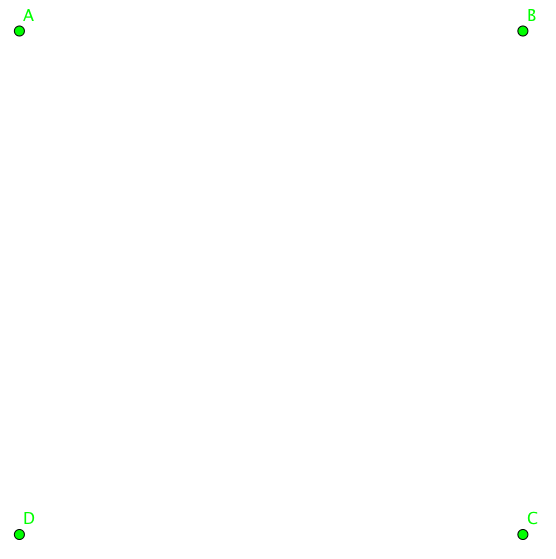
\includegraphics[width=\linewidth]{layer1square}
\caption{$P_1$ at $z=0$}\label{fig:layer1}
\end{subfigure}\hspace{10 mm}
\begin{subfigure}[b]{.25\linewidth}
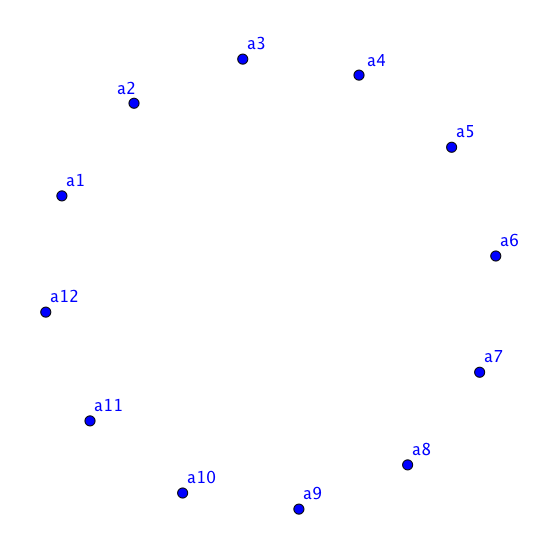
\includegraphics[width=\linewidth]{layer2regular}
\caption{$P_2$ at $z = \epsilon$}\label{fig:layer2}
\end{subfigure}\hspace{10 mm}
\begin{subfigure}[b]{.25\linewidth}
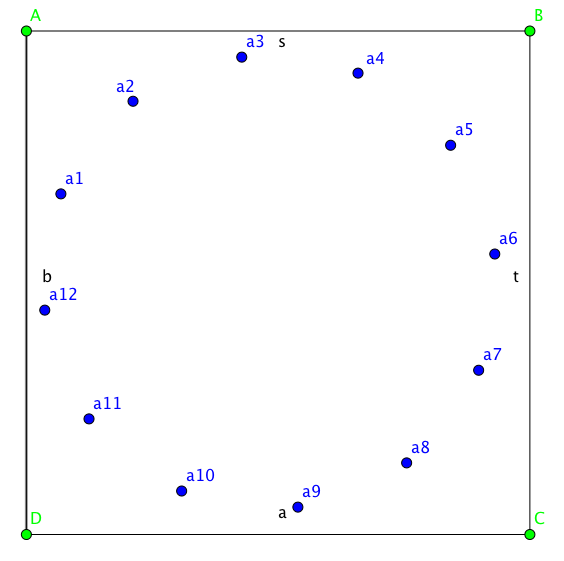
\includegraphics[width=\linewidth]{layer1and2}
\caption{$P_1, P_2$ projected}\label{fig:layer1and2}
\end{subfigure}
\caption{2D depiction of points in $P_1$ and $P_2$, ignoring $z$ coordinates}
\label{fig:lower_bound_construction_overview}
\end{figure}

$P_1$ contains 4 points that form a square, with coordinates, $(0,0)$, $(0,1)$, $(1, 0)$, $(1, 1)$, as shown in figure~\ref{fig:layer1}. $P_2$ has $n = 10f(4)$ points, forming a regular polygon that is centered around $(0.5, 0.5)$ with $x, y$ coordinates between 0 and 1, as shown in figure~\ref{fig:layer2}. So if we ignore the $z$ coordinates, $P_2$ is contained inside $P_1$, as shown in figure~\ref{fig:layer1and2}. Order the points in $P_2$ anti-clockwise, $a_1, ..., a_n$. Group the points into disjoint sets of 5 consecutive points. So the first group will have the points $a_1, ..., a_5$, the second group has the points $a_6, ..., a_{10}$, etc. For each group of 5 points in $P_2$ we will construct $m = 10f(n+4) = 10f(10f(4) + 4)$ points in $P_3$.

\begin{figure}[!htb]
\centering
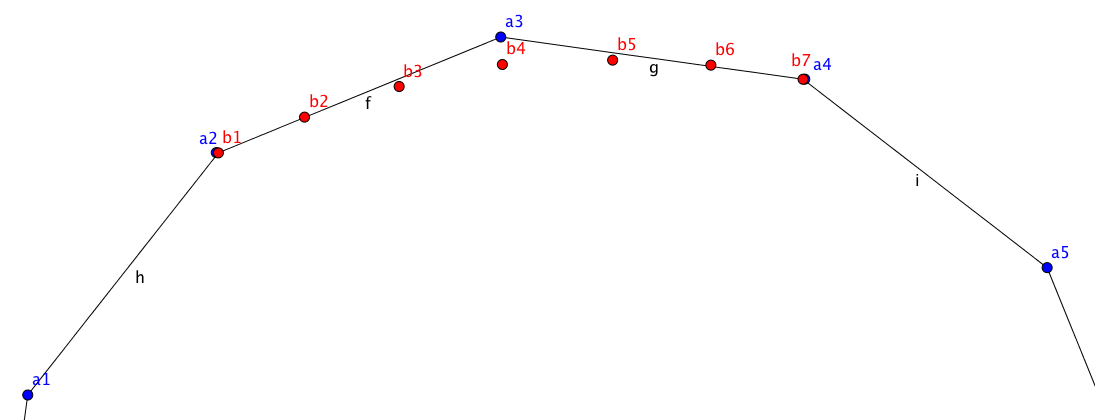
\includegraphics[width=0.6\linewidth]{layer3points}
\caption{Red points are in $P_3$, blue in $P_2$}
\label{fig:layer3}
\end{figure}

WLOG consider $a_1, ..., a_5$ in $P_2$. For each such group, we will add points $b_1, ..., b_m$ to $P_3$. Ignoring $z$ coordinates, we set $b_1 = a_2$, $b_m = a_4$. All the points $b_1, ..., b_m$ will be contained in the triangle defined by $a_2, a_3, a_4$. The points $b_1, ..., b_m$ are equally spaced, and form equal angles that are less than 180 degrees. We illustrate this construction in figure~\ref{fig:layer3}. We note that by our construction $P_1, P_2, P_3$ are meaningful. We choose the smallest $\epsilon$ such that $P_1, P_2, P_3$ are $\epsilon$ meaningful. Now, we will prove the theorem.
\\

Suppose we run $A$ on $P_1 @ P_2$. Ignoring $z$ coordinates, $P_2$ is contained inside $P_1$. Since the $z$ coordinates of points in $P_1$ and $P_2$ are $0$ and $\epsilon$ respectively, $P_1$ is an $\epsilon$-approximate convex hull for $P_1 @ P_2$. So OPT$(P_1 @ P_2, \epsilon) \leq 4$. Since $A$ is always-1-OPT, it can keep at most $f(4)$ points in $P_1 @ P_2$. $P_2$ has a total of $10f(4)$ points, which we divided into $2f(4)$ groups of $5$ points. So $A$ did not store any points in at least $f(4)$ of these groups, call these the unselected groups in $P_2$.
\\

Now suppose we run $A$ on $P_1 @ P_2 @ P_3$. For each of the $f(4)$ unselected groups in $P_2$, we selected $m = 10f(n+4)$ points in $P_3$. $A$ has to select all the corresponding $m$ points in $P_3$. To prove this, suppose for the sake of contradiction we don't have to select some corresponding point $p$ in $P_3$. $p$ cannot be written as an $\epsilon$-approximate convex combination of selected points in $P_2$, because the $z$ coordinate of $p$ and points in $P_2$ differ by $\epsilon$ \emph{and} if we ignore $z$ coordinates (projecting to the plane $z = 0$) $p$ corresponds to an unselected group and so does not lie inside the convex hull of selected points in $P_2$. Furthermore, since we selected $P_3$ to be $\epsilon$-meaningful, $p$ cannot be written as an $\epsilon$-approximate convex combination of other points in $P_3$.
\\

Summing over unselected groups, this means that $A$ must keep $f(4)m = 10f(4)f(n+4)$ points in $P_3$. The optimal approximate hull of $P_1 @ P_2 @ P_3$ is much smaller: we can simply store all the points in $P_1$ and $P_2$ giving us a total of $n + 4$ points. So OPT$(P_1 @ P_2 @ P_3, \epsilon) \leq n + 4$, which means $A$ is allowed to keep at most $f(n+4)$ points. $10f(4)f(n+4) > f(n+4)$ so we have a contradiction. 

\end{proof}

\begin{theorem}
For all $r \in \mathbb{Z}^+$, there does not exist an always-$r$-OPT streaming algorithm in $\mathbb{R}^3$.
\label{thm:alwaysropt}
\end{theorem}

\begin{proof}
The construction is similar to theorem~\ref{thm:alwaysopt}, with a few differences. Instead of constructing 3 sets of points $P_1, P_2, P_3$, we construct $r+1$ sets of points $P_1, ..., P_{r+1}$. All points in $P_i$ will have $z$ coordinate $(i-1)\epsilon$. For the $x, y$ coordinates, the construction of $P_{i+1}$ for $i \geq 2$ is similar to the construction of $P_3$ in theorem~\ref{thm:alwaysopt}. We group $P_i$ into disjoint groups of $5$ points. Let $n_i$ be the total number of points in $P_1, ..., P_i$. For each group in $P_i$ we add $10f(n_i)$ points in $P_{i+1}$. We then choose $\epsilon$ so that $P_i$ is $r\epsilon$ meaningful for all $i$.
\\

The proof of the construction is also similar to theorem~\ref{thm:alwaysopt}, except we apply the argument inductively. We can show that for each $i$, there exists an unselected group of 5 points in $P_i$, and further if we project onto $z=0$ the unselected group would be at least distance $r\epsilon$ outside the convex hull of points we select in $P_2, ..., P_{i-1}$. At $P_{r+1}$, this will give us an unselected point that is not an $r\epsilon$-approximate convex combination of selected points.
\end{proof}

\begin{corollary}
The above proof holds for both deterministic and randomized algorithms since it first presents a construction, and then cases on a particular run of the algorithm. It does not assume the algorithm runs the same way each time.
\end{corollary}

\begin{corollary}
For all $r \in \mathbb{Z}^+$ and $n \geq 3$, there does not exist an always-$r$-OPT streaming algorithm in $\mathbb{R}^n$.
\end{corollary}

\begin{proof}
If $n \geq 3$, $\mathbb{R}^n$ contains a 3D subspace so we can use the previous construction.
\end{proof}

% \section{Random Order Lower Bound}

% The 2D algorithm we give in chapter 4 works with high probability assuming that the points in the point stream come in a random order. In particular, every permutation of the stream $P$ must be equally likely. This assumption is very often true if the data is generated from a certain process (if the data points are i.i.d.). A natural question is whether assuming random order can give us an always-OPT streaming algorithm.

% \begin{definition}
% We say a streaming algorithm $A$ is \emph{weak random order always-OPT} if there exists $r \in \mathbb{Z}^+$ and a function $f : \mathbb{Z}^+ \to \mathbb{Z}^+$ such that: given an arbitrary point stream $P$, for at least 1\% of the permutations of $P$, if $A$ is run on the permutation, then after processing all points in $P$, $A$ keeps an $r\epsilon$-approximate convex hull of $P$ with size at most $f(\mbox{OPT}(P, \epsilon))$.
% \end{definition}

% \begin{theorem}
% For all $n \geq 3$, there does not exist a weak random order always-OPT streaming algorithm in $\mathbb{R}^n$.
% \end{theorem}

% \begin{proof}
% Filling it out now.
% % Given a point stream $P$ containing $n$ points ordered $p_1, ..., p_n$, we can essentially create a new point stream $P'$ that ``forces" the points to come in the same order as in $P$. Then we can use the construction in  }.
% % \\

% % We construct $P'$ inductively. For the base case, we will add 1 copy of the point $p_n$ to $P'$. For the inductive case, consider some $1 \leq i < n$. Suppose $P'$ currently has $m$ points (it only contains points $p_{i+1}, ..., p_n$ but it will contain multiple copies of most of these points). We will add $100nm$ copies of the point $p_i$ to $P'$.
% % \\

% % If $P'$ is randomly permuted, the probability that the first point in $P'$ is $p_1$ is $\geq 1 - \frac{1}{100n}$. So the probability that the first point is not $p_1$ is $\leq \frac{1}{100n}$. Intuitively, this is because most of the points in $P'$ are simply copies of $p_1$, so with very high probability we will see $p_1$ first. Continuing this process, and applying union bound, the probability the points do not come in the order $p_1, ..., p_n$ is at most $\frac{1}{100}$.
% % \\

% % So we can take the point stream $P_1 @ P_2 @ ... @ P_{r+1}$ we constructed in theorem~\ref{thm:alwaysropt} and apply this transformation to get a new point stream $P'$. For at least $\frac{99}{100}$ of the permutations of $P'$ the points will appear in the desired order
% % This means that for at least $\frac{99}$
% \end{proof}

\section{MAX-OPT Lower Bound}

We now show that even using a weaker notion of OPT, MAX-OPT, does not trivialize our problem.

\begin{definition}
Suppose that points in a point stream $P$ are ordered from 1 to $n$. Let $P_{i:j}$ denote a point stream containing the points from index $i$ to index $j$, inclusive of both index $i$ and $j$. In particular, $P_{1:n}$ is the entire point stream $P$.
\end{definition}

\begin{definition}
We define \emph{MAX-OPT$(P, \epsilon)$} as $\max_{1 \leq i \leq n} \mbox{OPT}(P_{i:n}, \epsilon)$, that is, the max of OPT taken over all prefixes of $P$.
\end{definition}

MAX-OPT is at least as large as OPT. Moreover, when we run an always-OPT algorithm $A$ on a stream $P$, at some point its memory usage must be a function of MAX-OPT. This is because MAX-OPT is OPT for some prefix $P'$ of $P$, and $A$ would have received the prefix $P'$ at some point. This is not too different from an algorithm that uses MAX-OPT space while processing the entire stream. The total (maximum) amount of memory we need to allocate to both algorithms is the same. So a natural question is whether a streaming algorithm can be competitive with MAX-OPT (independent of the number of points received so far). We define an always-MAX-OPT algorithm like an always-OPT algorithm, replacing OPT with MAX-OPT.

\begin{definition}
We say a streaming algorithm $A$ is \emph{always-MAX-OPT} if there exists $r \in \mathbb{Z}^+$ and a function $f : \mathbb{Z}^+ \to \mathbb{Z}^+$ such that: if $A$ is run on an arbitrary point stream $P$, then after processing all points in $P$, $A$ keeps an $r\epsilon$-approximate convex hull of $P$ with size at most $f(\mbox{MAX-OPT}(P, \epsilon))$.
\end{definition}

\begin{theorem}
For all $n \geq 3$, there does not exist an always-MAX-OPT streaming algorithm in $\mathbb{R}^n$.
\end{theorem}

\begin{proof}
The same construction and proof in theorem~\ref{thm:alwaysropt} works.
\end{proof}

\section{Almost Always OPT}

The algorithm we give in chapter 5 is of a slightly different nature.

\begin{definition}
A streaming algorithm $A$ is \emph{almost always OPT} if there exists a function $f : \mathbb{Z}^+ \to \mathbb{Z}^+$ such that the following holds. Suppose $A$ is given $k \in \mathbb{Z}^+$ in advance, and is run on an arbitrary point stream $P$ with $\mbox{OPT}(P, \epsilon) \leq k$. At any point, $A$ is allowed to keep at most $f(k)$ points. After processing all points in $P$, $A$ keeps an $\epsilon$-approximate convex hull of $P$.
\end{definition}

\begin{theorem}
There does not exist an almost always OPT streaming algorithm in $\mathbb{R}^3$.
\label{thm:almostalwaysopt}
\end{theorem}

\begin{proof}
We first prove this for a deterministic algorithm and then sketch out how to extend the proof to a randomized algorithm. Assume for the sake of contradiction that there exists a deterministic almost always OPT streaming algorithm in $\mathbb{R}^3$.
\\

We modify the construction in theorem~\ref{thm:alwaysopt}. We construct 3 points sets $P_1$, $P_2$, $P_3$. Points in $P_1, P_2, P_3$ have $z$-coordinates $0, \epsilon, 2\epsilon$ respectively, so we describe their $x, y$ coordinates. $P_1$ contains 4 points $(0,0), (0,1), (1,0), (1,1)$ like in theorem~\ref{thm:alwaysopt}. $P_2$ is a regular polygon centered around $(0.5, 0.5)$ with $x, y$ coordinates between $0$ and $1$. However, $P_2$ contains $n = 10f(7)$ points. We group the points in $P_2$ into consecutive groups of 5 like in theorem~\ref{thm:alwaysopt}.
\\

We will set $k=7$ and run $A$ on $P_1 @ P_2$. $A$ is allowed to keep at most $f(7)$ points, so it can keep at most $f(7)$ points in $P_2$. However, $P_2$ had $2f(7)$ groups of 5 points. So at least one of the groups is unselected, suppose the points in one of these groups are $a_1, ..., a_5$. For this group of 5 points, we use the construction we used in theorem~\ref{thm:alwaysopt} shown in figure~\ref{fig:layer3}, except we add $2f(7)$ (instead of $10f(10f(4) + 4)$) points to $P_3$. If we project all points onto the plane at $z = 0$ then $P_3$ will be contained inside the triangle defined by $a_2, a_3, a_4$.
\\

We define $\epsilon$ to be the smallest value such that $P_1, P_2, P_3$ are $\epsilon$-meaningful. Note that the choice of $\epsilon$ is independent of which group was unselected, since $P_2$ is a regular polygon and is therefore symmetric. Now, suppose we run $A$ on the stream $P_1 @ P_2 @ P_3$. $P_1 \cup \{ a_2, a_3, a_4 \}$ forms an $\epsilon$-approximate convex hull of $P_1 @ P_2 @ P_3$ so OPT$(P_1 @ P_2 @ P_3, \epsilon) \leq 7$. Since $A$ is almost always OPT, it must find a way to keep an $\epsilon$-approximate convex hull of $P_1 @ P_2 @ P_3$ of size $\leq f(7)$. However, $A$ must choose all points in $P_3$, because their distance from selected points in $P_1$ and $P_2$ is greater than $\epsilon$, and $P_3$ is $\epsilon$-meaningful. So $A$ must store $2f(7)$ points, a contradiction.
\\

This proof can be extended to show that there does not exist a randomized almost always OPT streaming algorithm in $\mathbb{R}^3$.
\end{proof}

Note that even if we use MOX-OPT instead of OPT, theorem~\ref{thm:almostalwaysopt} still holds.

\section{Limitations}

We believe that lower bounds should be treated as specific hardness results that guide research but that should not be generalized out of context or discourage work on a problem. The lower bounds we gave in this chapter have limitations, some of which are given below.

\begin{enumerate}
\item None of our lower bounds hold for 2D. Empirically, finding an always OPT or almost always OPT algorithm in 2D is a difficult problem, however it might not be impossible.
\item There might exist algorithms in higher dimensions that have a dependency on $\log{\frac{1}{\epsilon}}$ or $\log{n}$. For example we could be competitive with $\mbox{OPT} \cdot \log{\frac{1}{\epsilon}}$, which would still be a very useful result.
\item We could add reasonable assumptions, for example the assumption that the points come in a random order, which we do in chapter 4.
\item We might be able to relax the problem in useful ways and find solutions to those relaxations, like the relaxation we discuss in chapter 5.
\end{enumerate}
